% FILLED (fill batch): process ② Deceleration — AD/ELENA energy ladder.
%   folds stdlib rel_kinetic_from_p / rel_p_from_kinetic (PR #1014) + the
%   AD-in/AD-out/ELENA-out rungs + the p->T->p roundtrip identity + the two
%   negative controls, from companion/verify-ledger.json.
\section{Deceleration --- the AD/ELENA Relativistic Energy Ladder}
\label{app:deceleration}

This appendix is the full data record for pipeline process
\textcircled{\scriptsize 2}. We tabulate the Antiproton Decelerator / ELENA
momentum ladder \citep{maury1997ad,maury2014elena}, the relativistic
energy--momentum relation evaluated at each rung, the round-trip
$p\!\to\!T\!\to\!p$ closure, and the two deterministic negative controls.
Every digit traces to PR~\#1014 and the atoms in
\texttt{companion/verify-ledger.json}.

% -------------------------------------------------------------------------
\subsection{The relativistic energy--momentum relation}
\label{app:decel-rel}

After production at GeV momenta, the antiproton beam must be slowed to the
keV (and ultimately sub-eV) energies a trap can hold. The deceleration is a
ladder of storage-ring steps; at each rung the kinetic energy is fixed by the
relativistic invariant $E^2=(pc)^2+(m_pc^2)^2$ with $E=T+m_pc^2$, giving the
forward map
\begin{equation}
T(p) \;=\; \sqrt{(pc)^2 + (m_pc^2)^2}\;-\;m_pc^2 ,
\label{eq:decel-T}
\end{equation}
and its exact inverse
\begin{equation}
p(T) \;=\; \frac{1}{c}\sqrt{T^2 + 2\,T\,m_pc^2}
       \;=\; \frac{1}{c}\sqrt{(T+m_pc^2)^2-(m_pc^2)^2}.
\label{eq:decel-p}
\end{equation}
Eqs.~\eqref{eq:decel-T}--\eqref{eq:decel-p} are an exact inverse pair, so the
round-trip $p\to T\to p$ must reproduce the input momentum to machine
precision --- a built-in self-consistency atom (below). In the
ultra-relativistic limit $pc\gg m_pc^2$, $T\to pc$; in the non-relativistic
limit $pc\ll m_pc^2$, $T\to (pc)^2/2m_pc^2$ (the dropped $T^2$ term that the
negative control probes).

% -------------------------------------------------------------------------
\subsection{The AD/ELENA ladder rungs}
\label{app:decel-ladder}

CERN's AD takes $\sim$3.57\,GeV/$c$ antiprotons from the production target
and decelerates them to $\sim$100\,MeV/$c$; ELENA then takes the AD output
down to $\sim$13.7\,MeV/$c$ ($T=0.1$\,MeV)
\citep{maury1997ad,maury2014elena}. Table~\ref{tab:decel-rungs} gives the
three registered rungs and the round-trip identity, spanning $\sim$5 decades
in kinetic energy; the ladder is plotted in Fig.~\ref{fig:decel-app}.

\begin{table}[h]
\centering
\small
\setlength{\tabcolsep}{5pt}
\begin{tabular}{@{}l l r r r l@{}}
\toprule
\textbf{rung / atom} & \textbf{args} & \textbf{expected} & \textbf{observed} & $|\Delta|$ & \textbf{tier} \\
\midrule
AD input \verb|rel_kinetic_from_p|   & (3500.0)  & $2685.31$ & $2685.31$ & $0$       & \tierGreen \\
AD output \verb|rel_kinetic_from_p|  & (100.0)   & $5.3139$  & $5.3139$  & $0$       & \tierGreen \\
ELENA out \verb|rel_p_from_kinetic|  & (0.1)     & $13.6991$ & $13.6991$ & $0$       & \tierGreen \\
roundtrip \verb|rel_p_from_kinetic|  & (5.3139)  & $100.0$   & $100$     & $7.4\times10^{-13}$ & \tierGreen \\
\bottomrule
\end{tabular}
\caption{Process \textcircled{\scriptsize 2} deceleration rungs
(\texttt{companion/verify-ledger.json}, PR~\#1014). The first three rows are
the AD-in / AD-out / ELENA-out ladder steps via
Eqs.~\eqref{eq:decel-T}--\eqref{eq:decel-p}; the last row is the round-trip
$p\!\to\!T\!\to\!p$ self-consistency identity, closing to
$|\Delta|=7.4\times10^{-13}$ (the residual is a single \texttt{sqrt}
round-off, not a modelling error).}
\label{tab:decel-rungs}
\end{table}

\begin{figure}[h]
\centering
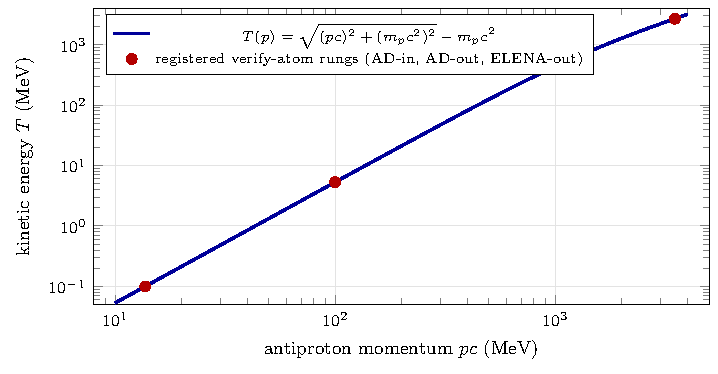
\includegraphics[width=0.80\linewidth]{figures/fig05_decel_ladder.pdf}
\caption{The AD/ELENA relativistic deceleration ladder
$T(p)=\sqrt{(pc)^2+(m_pc^2)^2}-m_pc^2$ (log--log), spanning $\sim$5 decades
in kinetic energy from the AD input ($pc=3500$\,MeV, $T=2685$\,MeV) to the
ELENA output ($T=0.1$\,MeV). The marked points are the three registered
\tierGreen\ rungs of Table~\ref{tab:decel-rungs}; the curve through them is
the exact relativistic relation, not a fit. Atoms
\texttt{rel\_kinetic\_from\_p} / \texttt{rel\_p\_from\_kinetic} (PR~\#1014).}
\label{fig:decel-app}
\end{figure}

% -------------------------------------------------------------------------
\subsection{Negative controls}
\label{app:decel-controls}

Two deterministic negative controls confirm the verifier is
result-agnostic: a wrong-answer probe on the AD-in rung, and a
non-relativistic-limit probe on the ELENA rung that drops the $T^2$ term of
Eq.~\eqref{eq:decel-p}. Both return \textsc{Falsified}
(Table~\ref{tab:decel-controls}).

\begin{table}[h]
\centering
\small
\begin{tabular}{@{}l l r r r l@{}}
\toprule
\textbf{control} & \textbf{args} & \textbf{expected} & \textbf{observed} & $|\Delta|$ & \textbf{tier} \\
\midrule
\verb|rel_kinetic_from_p| (wrong answer)   & (3500.0) & $2700.0$  & $2685.31$ & $14.69$ & \tierRed \\
\verb|rel_p_from_kinetic| (non-rel.\ limit)& (0.1)    & $13.6987$ & $13.6991$ & $4\times10^{-4}$ & \tierRed \\
\bottomrule
\end{tabular}
\caption{The two deterministic \textsc{Falsified} controls for process
\textcircled{\scriptsize 2} (\texttt{companion/verify-ledger.json},
PR~\#1014). The second probes the non-relativistic approximation
$p\approx\sqrt{2Tm_pc^2}/c$: at $T=0.1$\,MeV the dropped $T^2$ term shifts
$p$ by $4\times10^{-4}$\,MeV/$c$, large enough to falsify at
$\varepsilon=10^{-9}$ --- exactly the relativistic correction the full
formula keeps.}
\label{tab:decel-controls}
\end{table}

\begin{lstlisting}
verify --expr rel_kinetic_from_p(3500.0)=2685.31
  calc   = 2685.31 ~ expected 2685.31 (|Delta|=0.0 <= eps=1e-9)
  tier   = SUPPORTED-NUMERICAL (hexa-native libm-class recompute)
verify --expr rel_p_from_kinetic(5.3139)=100.0   # p->T->p roundtrip
  calc   = 100.000 ~ expected 100.0 (|Delta|=7.39e-13 <= eps=1e-9)
  tier   = SUPPORTED-NUMERICAL (hexa-native libm-class recompute)
verify --expr rel_kinetic_from_p(3500.0)=2700.0  # negative control
  calc   = 2685.31 != expected 2700.0 (|Delta|=14.69 > eps=1e-9)
  tier   = FALSIFIED (controlled negative; verifier is result-agnostic)
\end{lstlisting}

% -------------------------------------------------------------------------
\subsection{Honest scope}
\label{app:decel-scope}

This appendix closes the \emph{kinematics} of each rung --- the exact
momentum$\leftrightarrow$kinetic-energy map and its round-trip closure --- not
the deceleration \emph{efficiency} or the stochastic/electron cooling between
rungs, which depend on ring-specific cooling hardware out of scope here. The
ladder's three numerical anchors are representative AD/ELENA operating points
\citep{maury1997ad,maury2014elena}, not a sourced shift-by-shift machine log.
